
\section{Model Diagnostics for Roy's Models}

Further to previous work, this section revisits case-deletion and residual diagnostics, and explores how approaches devised by  \citet{Galecki} can be used to appraise Roy's model. These authors specifically look at Cook's Distances and Likelihood Distances.
%	For the Roy Model, Cook's Distances may also be generated using the \textbf{\textit{predictmeans}}
%	





\begin{figure}[h!]
	\centering
	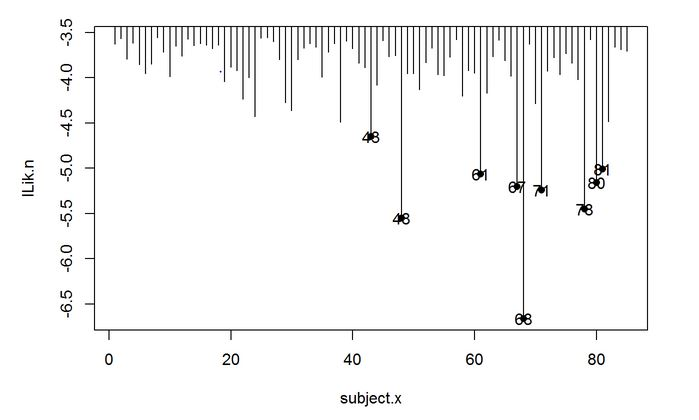
\includegraphics[width=0.7\linewidth]{images/LogLik-JS-Roy}
	\caption{}
	\label{fig:LogLik-JS-Roy}                                                                                         
\end{figure}





\citet{ARoy2009} establishes the equivalence of repeatability and within-item variability, and hence precision.  The method with the smaller within-item variability can be deemed to be the more precise.                                              d
A useful approach is to compute the confidence intervals for the ratio of within-item standard deviations, which is interpreted in the usual manner.
%

\citet[pb 93-95]{PB} give a description of how confidence intervals for the variance components are computed. Furthermore a complete set of confidence intervals can be computed to complement the variance component estimates. What is required is the computation of the variance ratios of within-item and between-item standard deviations.

A naive approach would be to compute the variance ratios by relevant F distribution quantiles. However, the question arises as to the appropriate degrees of freedom. Bootstrap methods for computing confidence intervals may be considered.

Further to previous work, this section revisits case-deletion and residual diagnostics, and explores how approaches devised by \citet{Galecki} can be used to appraise Roy's model. These authors specifically look at Cook's Distances and Likelihood Distances.
%For the Roy Model, Cook's Distances may also be generated using the \textbf{\textit{predictmeans}}

Applying the core principals of this methods to method comparison problem, case deletion diagnostics are used on the variance components of the Roy's model, specifically the ratio of between-subject variances and the within-subject covariances respectively.
\[ \mbox{WSVR} = \frac{\sigma^2_1}{\sigma^2_2} \phantom{makespace}  \mbox{BSVR} = \frac{g^2_1}{g^2_2} \]
These variance ratios are re-computed for each case removed, and may be analysed seperately or jointly for outliers, using standard techniques, such as the Grubbs tests.


The WSVR values are plotted against the corresponding BSVR values, with commonly used bivariate methods may be applied jointly to the both sets of data sets, e.g Mahalanobis distances. Confidence ellipses can be superimposed over the plot with minimal effort. Two ellipses are generated by this technique, a 50\% and 97.5\% confidence ellipse respectively. Outlying cases are idenified by the plot. Subject 68 is the most prominent case.

The subjects were ranked by Mahalanobis distance, with the top 10 being presented in the following table. Both sets of ratio are addtionally expressed as a ratio of the full model variance ratios.
\begin{center}
	\begin{tabular}{|c|c|c|c|c|c|}
		\hline
		Subject (u) &  MD & WSVR$_{(u)}$ & WSVR (\%) & BSVR$_{(u)}$   & BSVR (\%)     \\ \hline \hline
		68 & 44.7284   & 1.3615  & 0.9132   & 1.0353  & 0.9849 \\ \hline
		30 & 16.7228   & 1.5045  & 1.0092   & 1.1024  & 1.0487 \\ \hline
		71 & 11.5887   & 1.5210  & 1.0202   & 1.0932  & 1.0400 \\ \hline
		80 & 11.0326   & 1.4796  & 0.9925   & 1.0114  & 0.9621 \\ \hline
		38 & 10.3671   & 1.5011  & 1.0069   & 1.0917  & 1.0385 \\ \hline
		67 & 10.1940   & 1.4308  & 0.9598   & 1.0514  & 1.0002 \\ \hline
		43  & 7.6932   & 1.4385  & 0.9649   & 1.0511  & 0.9999 \\ \hline
		72  & 4.7350   & 1.4900  & 0.9995   & 1.0262  & 0.9762 \\ \hline
		48  & 4.4321   & 1.4950  & 1.0028   & 1.0280  & 0.9779 \\ \hline
		29  & 4.3005   & 1.4910  & 1.0001   & 1.0769  & 1.0244 \\ \hline
	\end{tabular}
\end{center}
From this table one may conclude that subjects 72, 48 and 29 are not particularly influential. Interestingly Subject 78, which was noticeable in the case deletion diagnostics for fixed effects, does not feature in this table.

\begin{figure}[h!]
	\centering
	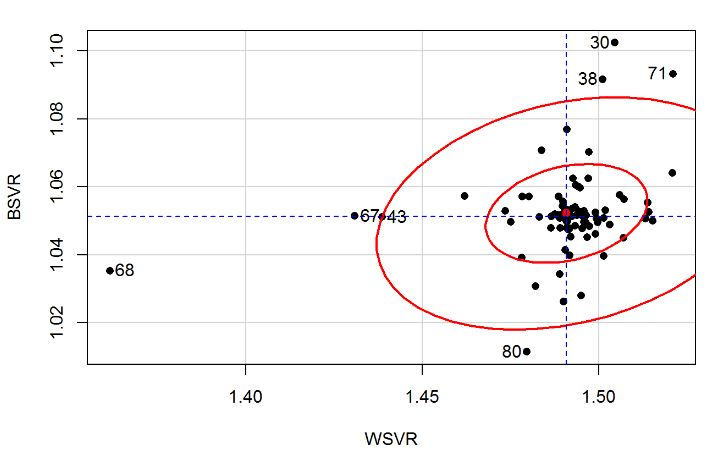
\includegraphics[width=0.9\linewidth]{08-plot1}
	\caption{Identification of Prominent Observations}
	\label{fig:08-plot1}
\end{figure}
\end{document}